\documentclass[a4paper, 12pt,oneside]{article}
\usepackage{graphicx} % Required for inserting images
\usepackage[top=2.5cm, bottom=2cm, left=2cm, right=2cm]{geometry}
\usepackage[french]{babel}  % Définit le français comme langue principale
\usepackage[utf8]{inputenc}  % Gère les accents et caractères spéciaux (si nécessaire)
\usepackage[T1]{fontenc}
\usepackage[colorlinks,bookmarks=false,linkcolor=black,urlcolor=blue, citecolor=black]{hyperref}
\usepackage{units}
\usepackage{verbatim}
\usepackage{verbdef}% http://ctan.org/pkg/verbdef
\usepackage{amsmath}
\usepackage{amssymb}
\usepackage{wrapfig}
\usepackage{subcaption}
\usepackage{caption}
\usepackage{float}
\usepackage[export]{adjustbox}
\usepackage{upgreek}
\usepackage{hyperref}
%Pour changer la taille des titres de section et subsection. Ajoutez manuellement les autres styles si besoin.
\makeatletter
\renewcommand{\section}{\@startsection {section}{1}{\z@}%
             {-3.5ex \@plus -1ex \@minus -.2ex}%
             {2.3ex \@plus.2ex}%
             {\normalfont\normalsize\bfseries}}
\makeatother

\makeatletter
\renewcommand{\subsection}{\@startsection {subsection}{1}{\z@}%
             {-3.5ex \@plus -1ex \@minus -.2ex}%
             {2.3ex \@plus.2ex}%
             {\normalfont\normalsize\bfseries}}
\makeatother

\graphicspath{{Graphes/}}

\begin{document}
\title{\normalsize{Lab Work Report - Group N$^\circ$\\ XX - Experiment}}
\date{\normalsize{\today}}
\author{\normalsize{Name} 1\and \normalsize{Name 2}}

\begin{center}
\large\textbf{\sffamily Expérience N$^\circ$G7. Ultrasons}\\%
\large\sffamily Groupe N$^\circ$22: Armand Le Douarec, Maxime Chatelin\\%
\large\sffamily\today\quad   Assistant -  Enki Bendjoya \\%
\end{center}

\vspace{-0.25cm}
\section{Introduction}
\vspace{-0.25cm}

Avec des fréquences dépassant 30 kHz, bien au-delà de la limite de perception humaine fixée à 20 kHz [\ref{ref1}], les ultrasons ont suscité un vif intérêt dès leur découverte au XIXe siècle dans le cadre des études sur la propagation des ondes acoustiques [\ref{ref2}]. Ces vibrations inaudibles ont ouvert la voie à des avancées technologiques majeures grâce à leur capacité à se propager dans divers milieux tout en interagissant avec ceux-ci de manière prévisible et mesurable. Exploités dans des domaines tels que la médecine, où l’échographie permet une observation précise et non invasive des structures internes [\ref{ref3}], et l’industrie, où les sonars [\ref{ref4}]et les dispositifs d’inspection des matériaux [\ref{ref5}] sont devenus incontournables, les ultrasons jouent un rôle central dans des applications reposant sur l’analyse des échos qu’ils produisent. Ce travail s’inscrit dans cette dynamique et vise à étudier plusieurs propriétés fondamentales des ultrasons à travers une série d’expériences. La première étape consiste à analyser la réponse fréquentielle d’un transducteur récepteur pour caractériser sa sensibilité en fonction des fréquences. Ensuite, la vitesse du son dans un milieu sera déterminée à l’aide de méthodes utilisant des ondes continues et pulsées. Enfin, les phénomènes d’interférences acoustiques seront examinés, avec une attention particulière portée sur l’étude des battements, une manifestation temporelle résultant de la superposition de deux ondes de fréquences légèrement différentes.

\vspace{-0.25cm}
\section{Théorie}
\vspace{-0.25cm}

\paragraph{Ultrasons}

Les ultrasons sont ici générés grâce au phénomène de piézoélectricité [\ref{ref6}]. Ce dernier exploite les propriétés d’un matériau céramique placé entre deux électrodes, dans ce TP un résonateur piézoélectrique. Lorsqu’une tension alternative est appliquée aux électrodes, la céramique se déforme mécaniquement à des fréquences correspondant à la tension appliquée, produisant ainsi des oscillations ultrasonores. Ce phénomène repose sur la résonance, où le dispositif est réglé pour maximiser l’amplitude des vibrations à une fréquence précise. L’avantage de cette technologie réside dans sa réversibilité : le même transducteur peut détecter des ultrasons en convertissant les vibrations reçues en signaux électriques, permettant ainsi de l’utiliser alternativement comme émetteur ou récepteur.

\vspace{-0.25cm}
\paragraph{Mesure de la vitesse du son avec des ondes continues}

La vitesse du son $c$ peut être déterminée en exploitant la relation fondamentale qui lie la longueur d’onde $\lambda$, la fréquence $f$ et la vitesse du son [\ref{ref6}] : 

\vspace{-0.4cm}
\begin{equation}
c = \lambda \cdot f
\label{eq1}
\end{equation}
\vspace{-0.4cm}

Dans un montage utilisant des ondes continues, un émetteur est relié à un générateur de signal sinusoïdal, tandis qu’un récepteur capte l’onde et transmet le signal à un oscilloscope synchronisé avec l’onde émise. En modifiant progressivement la distance $d$ entre l’émetteur et le récepteur, les oscillations de l’onde défilent sur l’écran de l’oscilloscope. Une variation de $n$ périodes complètes correspond à une variation de distance donnée par [\ref{ref6}] :

\vspace{-0.25cm}
\begin{equation}
d = n \cdot \lambda
\label{eq2}
\end{equation}
\vspace{-0.35cm}

Ainsi, en effectuant un fit linéaire de cette distance $d$ par rapport à $n/f$ de l’onde émise, la vitesse $c$ peut être calculée par la formule [\ref{ref6}] :

\vspace{-0.1cm}
\begin{equation}
c = f \cdot \frac{d}{n}
\label{eq3}
\end{equation}
\clearpage

\vspace{-0.2cm}
\paragraph{Mesure de la vitesse du son avec des ondes pulsées}

Les ondes pulsées offrent une approche différente, en effet, une série d’impulsions ultrasonores est générée par un émetteur, réfléchie par une surface métallique située à une distance $d$, puis captée par un récepteur placé à côté de l'émetteur, donc aussi à une distance $d$ de la surface réfléchissante. Le temps $\Delta \tau$ nécessaire pour qu’une impulsion parcoure une distance totale de $2d$ est mesuré à l’aide d’un oscilloscope synchronisé avec le signal émis. En faisant varier $d$, il est possible d’obtenir une relation directe entre la distance parcourue et le temps de trajet, permettant de calculer la vitesse du son [\ref{ref6}] :

\vspace{-0.25cm}
\begin{equation}
c = \frac{2 \cdot \Delta d}{\Delta \tau}
\label{eq4}
\end{equation}
\vspace{-0.25cm}

\paragraph{Interférences temporelles entre deux ondes}

Lorsqu’un récepteur capte la superposition de deux ondes continues de fréquences légèrement différentes $f_1$ et $f_2$, un phénomène d’interférences appelé battement apparaît. L’amplitude $A(t)$ de l’onde résultante peut être exprimée par la somme des contributions des deux ondes [\ref{ref6}] :

\vspace{-0.2cm}
\begin{equation}
A(t) = A_1 \sin(2 \pi f_1 t + \phi_1) + A_2 \sin(2 \pi f_2 t + \phi_2)
\label{eq5}
\end{equation}

\noindent avec $A_1, A_2$ les amplitudes et $\phi_1, \phi_2$ les déphasages respectifs des ondes superposées. Dans le cas particulier où $A_1 = A_2 = A$ et $\phi_1 = \phi_2$, l’équation se simplifie pour devenir [\ref{ref6}] :

\begin{equation}
A(t) = 2A \cos \left( 2 \pi \frac{|f_1 - f_2|}{2} t \right) \sin \left( 2 \pi \frac{f_1 + f_2}{2} t \right)
\label{eq6}
\end{equation}

\noindent Cette équation met en évidence deux fréquences [\ref{ref6}] : 

\begin{equation}
f_{-} = \frac{|f_1 - f_2|}{2} \quad \text{et} \quad f_{+} = \frac{f_1 + f_2}{2}
\label{eq7}
\end{equation}

\noindent avec $f_-$ qui correspond à la fréquence de l’enveloppe, et $f_+$ la fréquence moyenne ou porteuse.

\section{Démarche expérimentale}

\paragraph{Réponse fréquentielle des transducteurs résonnants}

La fréquence de résonance d’un transducteur est déterminée en faisant varier la fréquence d’excitation dans une plage comprise entre $(35.70 \pm 0.05)$\,kHz et $(55.00 \pm 0.05)$\,kHz, grâce à la fonction "frequency sweep" d’un générateur de fonctions. L’émetteur, alimenté par ce signal, génère une onde ultrasonore captée par un récepteur placé à une distance fixe. Le signal reçu est redressé à l’aide d’un amplificateur et visualisé sur un traceur XY sur ordinateur. La tension de sortie, associée à la fonction "sweep out", est proportionnelle à la fréquence d’entrée, permettant de relier les amplitudes enregistrées aux fréquences correspondantes. Les pics d’amplitude identifiés sur l’oscilloscope révèlent les fréquences de résonance, où la réponse du transducteur est maximale. C'est à la principale fréquence de résonance que les expériences suivantes sont réalisées. Il est important de relever que les résultats ont d'abord été récupérés par le Traceur XY sous forme de potentiel. En observant la tension donnée par le logiciel pour les fréquences minimales et maximales affichées par le générateur de fonction, une régression linéaire a été faite permettant d'en déduire la fréquence du signal selon la tension perçue par le Traceur XY.

\vspace{-0.2cm}
\paragraph{Mesure de la vitesse du son en ondes continues}

Pour cette expérience, un émetteur est connecté à un générateur de fonctions réglé sur un signal sinusoïdal de fréquence $f = (40.20 \pm 0.05)$\,kHz. Le récepteur, placé en face, est relié à un oscilloscope dont le balayage horizontal est synchronisé avec le signal émis. La distance $d$ entre les transducteurs est ajustée progressivement, permettant d’observer le déplacement des oscillations sur l’écran. Les positions correspondant à des déplacements de $n$ périodes de l’onde sont notées, avec $n$ variant entre 1 et 20. Les variations de $d$ sont mesurées avec une précision de $\pm 0.5$\,mm. La vitesse du son $c_c$ est déterminé à partir de la pente du fit linéaire résultant.

\paragraph{Mesure de la vitesse du son en ondes pulsées}

Dans le cas des ondes pulsées, le générateur de fonctions est configuré en mode impulsions régulières, et l’amplificateur en mode redresseur. L’oscilloscope permet de mesurer le temps de retard $\Delta \tau$ du signal après un aller-retour sur une distance totale $2d$. En faisant varier la distance $d$, les temps de retard $\Delta \tau$ sont relevés pour des intervalles allant de $(1.0 \pm 0.2)$\,ms à $(9.0 \pm 0.2)$\,ms. Chaque intervalle $\Delta \tau = (1.0 \pm 0.2)$\,ms est utilisé pour calculer les variations correspondantes $2\Delta d$. La vitesse du son $c_p$ est déterminé à partir de la pente du fit linéaire résultant.

\paragraph{Interférences temporelles entre deux ondes}

Ce phénomène est étudié en utilisant deux émetteurs réglés à des fréquences légèrement différentes et un unique récepteur connecté à un oscilloscope. Les variations des fréquences $f_1$ et $f_2$ permettent d’explorer le phénomène des battements sur un oscilloscope.
\vspace{-0.5cm}
\section{Résultats}

\paragraph{Réponse fréquentielle des transducteurs résonnants}

\begin{wrapfigure}{H}{0.5\textwidth}
    \centering
    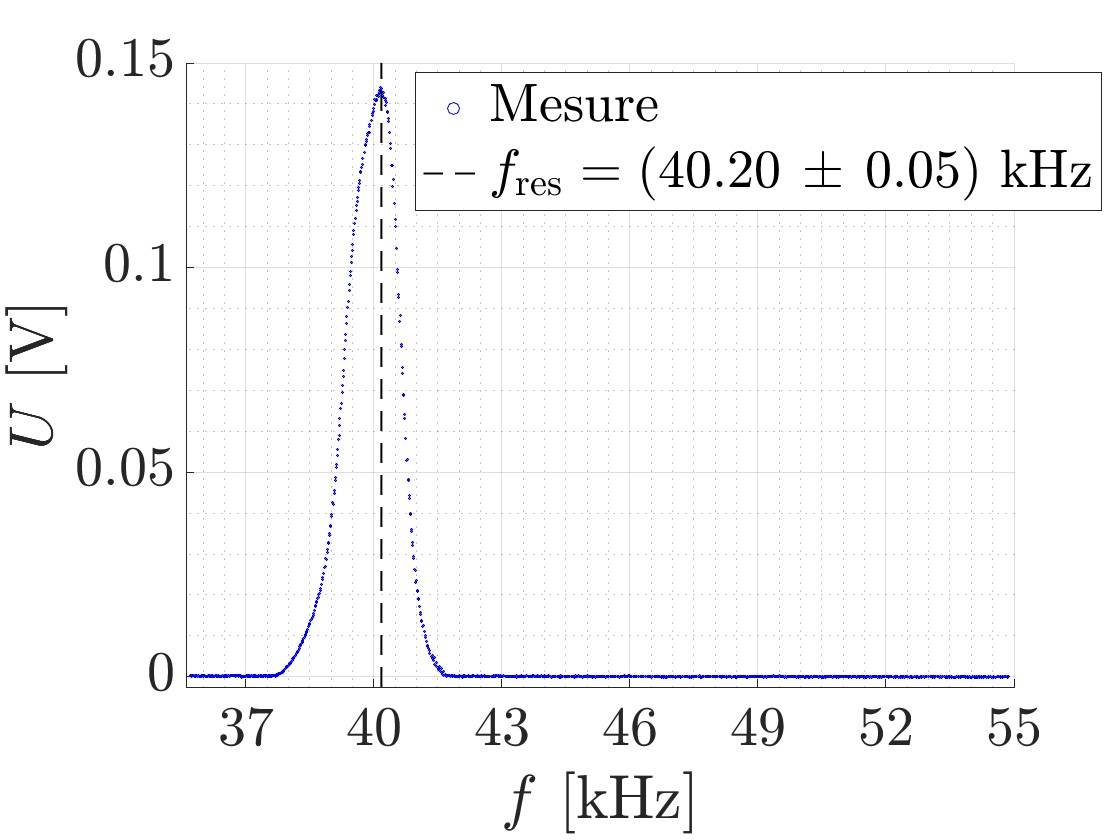
\includegraphics[width=1\linewidth]{Graphes_TP_F7/grph1.jpg}
    \captionsetup{justification=centering}
    \caption{Réponse fréquentielle du récepteur pour une fréquence variant de $f = (35.70 \pm 0.05)$\,kHz à $f = (55.00 \pm 0.05)$\,kHz}
    \label{fig1}
\end{wrapfigure}

La Fig.(\ref{fig1}) présente ici l'amplitude du signal perçu par le récepteur en fonction de la fréquence de l'émetteur variant entre $f = (35.70 \pm 0.05)$\,kHz et $f = (55.00 \pm 0.05)$\,kHz. Le graphique montre un unique pic de résonance à $f_{res} = (40.20 \pm 0.05)$\,kHz. 

\paragraph{Mesure de la vitesse du son avec des ondes continues}

La Fig.(\ref{fig2}) ci-dessous présente l’évolution de la distance $\Delta d$ entre l’émetteur et le récepteur en fonction de $\frac{n}{f}$, avec $f = (40.20 \pm 0.05)$\,kHz et $n$ allant de 1 à 20. Un ajustement linéaire des données expérimentales a permis de déterminer la pente $a = (348 \pm 1)$\,m$\cdot$s$^{-1}$. Or, la pente observée représente directement la vitesse du son comme le montre la relation (\ref{eq3}). Ainsi, le résultat donne $c_c = (348 \pm 1) \,$m$\cdot$s$^{-1}$.

\paragraph{Mesure de la vitesse du son avec des ondes pulsées}

La Fig.(\ref{fig3}) montre l’évolution de la distance $2 \Delta d$ parcourue par les ondes ultrasonores en fonction du temps de retard $\Delta \tau$, avec $\Delta d$ le déplacement de la distance entre les deux transducteurs et la plaque métallique réfléchissante. Encore une fois, une régression linéaire des données expérimentales a permis de déterminer la pente $a = (351 \pm 1) \, \text{m} \cdot \text{s}^{-1}$. De plus, il est possible de constater qu'avec la relation (\ref{eq4}), la vitesse du son correspond à cette pente ci, donnant donc $c_p = (351 \pm 1) \, \text{m} \cdot \text{s}^{-1}$

\begin{figure}[H]
    \centering
    \begin{minipage}{0.45\textwidth}
        \centering
        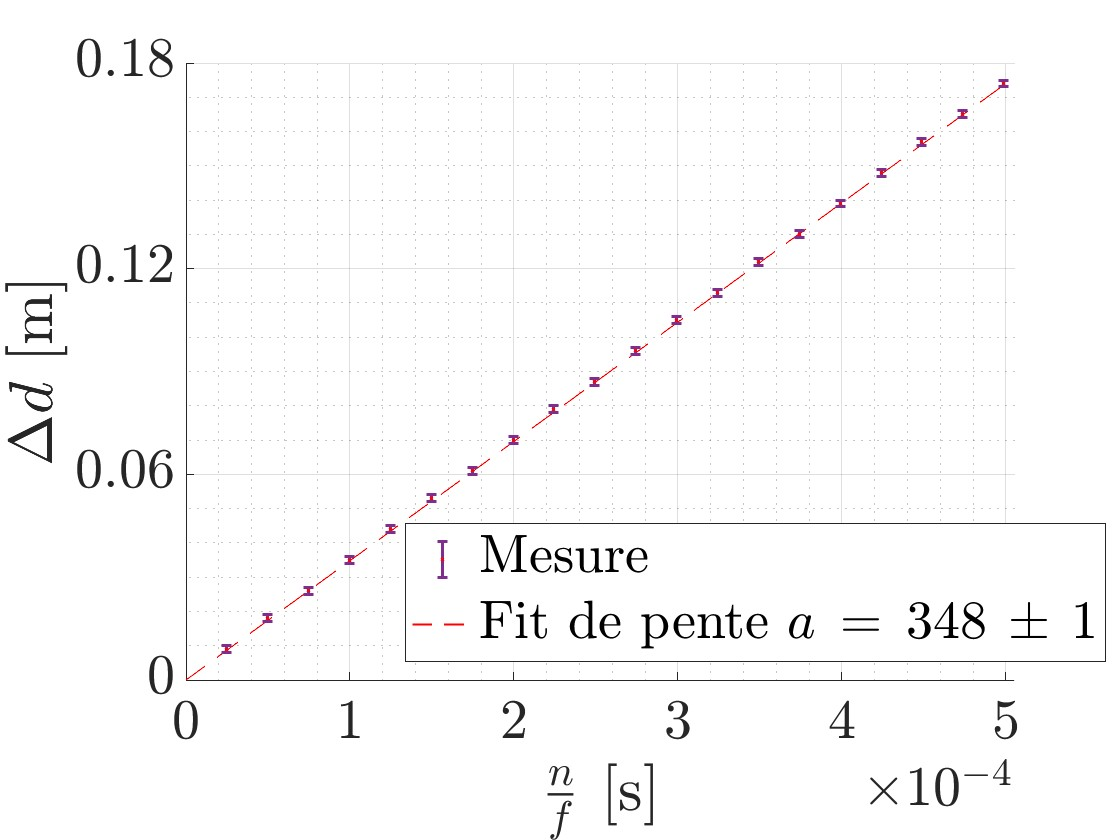
\includegraphics[width=\linewidth]{Graphes_TP_F7/grph2.jpg}
        \captionsetup{justification=centering}
        \caption{Graphique montrant un fit linéaire de pente $a=(348\pm1)$\,m$\cdot$s$^{-1}$ pour le déplacement $\Delta d$ en fonction de $\frac{n}{f}$ en ondes continues}
        \label{fig2}
    \end{minipage}
    \hfill
    \begin{minipage}{0.45\textwidth}
        \centering
        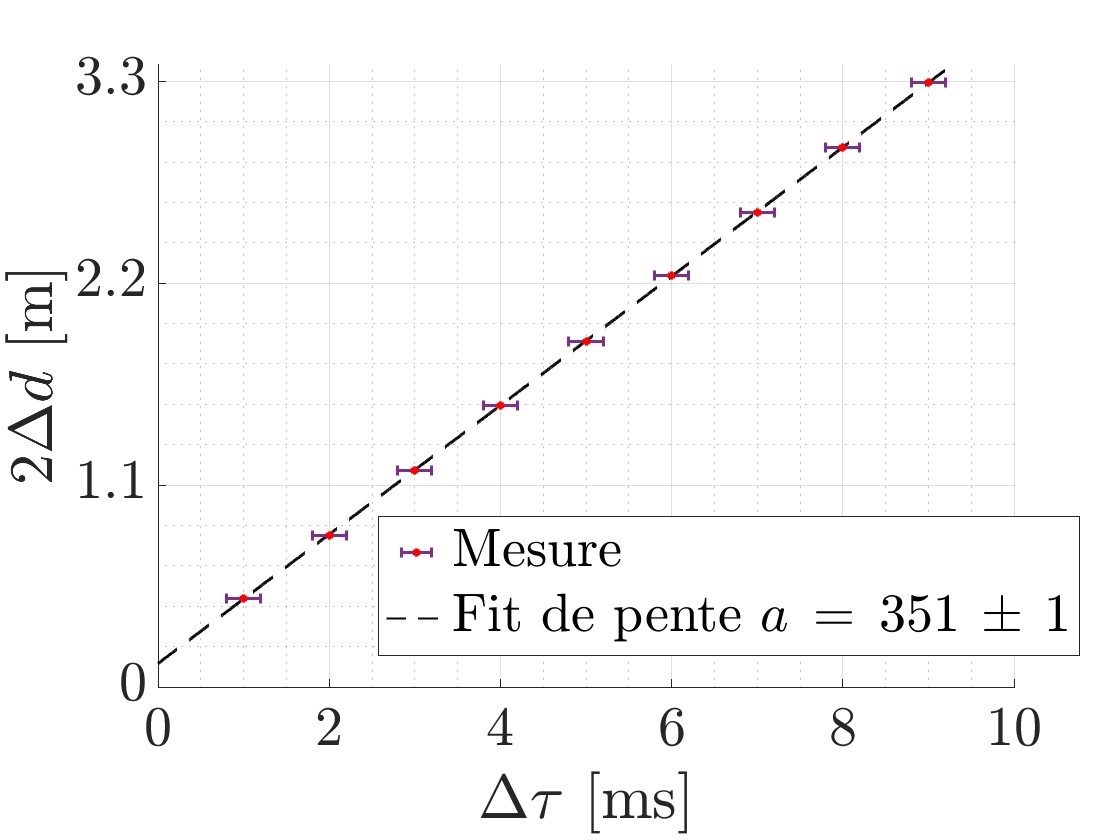
\includegraphics[width=\linewidth]{Graphes_TP_F7/grph3.jpg}
        \captionsetup{justification=centering}
        \caption{Graphique montrant un fit linéaire de pente $a=(351\pm1)$\,m$\cdot$s$^{-1}$ pour le déplacement $2\Delta d$ en fonction de $\Delta \tau$ en ondes pulsées}
        \label{fig3}
    \end{minipage}
\end{figure}
\vspace{-0.8cm}
\paragraph{Interférences temporelles entre deux ondes}

Le phénomène d’interférences a été étudié en superposant deux ondes sinusoïdales de fréquences légèrement différentes $f_1 = (40.10 \pm 0.05)$\,kHz et $f_2 = (40.30 \pm 0.05)$\,kHz, et d’amplitudes respectives $A_1$ et $A_2$. Ces ondes ont été émises simultanément par deux transducteurs distincts, puis captées par un récepteur unique, connecté à un oscilloscope. Trois configurations différentes, détaillées dans le Tab.(\ref{tab1}), ont été mises en œuvre pour visualiser l’effet les interférences, visibles sur les Fig.(\ref{fig4}), Fig.(\ref{fig5}) et Fig.(\ref{fig6}).

D'une part, les fréquences modulées théoriques $f_-^{\text{th}}$ et $f_+^{\text{th}}$ ont été calculées à l’aide de la relation (\ref{eq7}). D'autre part, les valeurs expérimentales de $f_-$, correspondant à la fréquence de l’enveloppe, et de $f_+$, la fréquence porteuse correspondant aux oscillations rapides à l’intérieur de l’enveloppe, ont été déterminées en mesurant la période de l’enveloppe et de l'onde porteuse directement sur l’oscilloscope. En effet, pour $f_-$, la Fig.(\ref{fig5}) et la  Fig.(\ref{fig6}) ont été utilisées et $f_+$ a été calculée à l'aide de la Fig.(\ref{fig4}).  Les résultats théoriques et expérimentaux pour chaque configuration sont présentés dans le Tab.(\ref{tab2}).

Les amplitudes théoriques $A_{\text{th}}$ ont été déterminées en utilisant les équations  (\ref{eq5}) et (\ref{eq6}). Quant aux amplitudes expérimentales, elles ont été mesurées directement en ordonnées sur l’écran de l’oscilloscope.

\begin{figure}[H]
    \centering
    \includegraphics[width=0.4\textwidth]{frequence.JPG}
    \captionsetup{justification=centering}
    \caption{Photo de l'oscilloscope pour la première configuration avec $f_1=(40.10\pm0.05)$\,kHz et $f_2=(40.30\pm0.05)$\,kHz, $A_1=A_2=(0.6\pm0.1)$\,V, time/div = 0.1\,ms et volt/div = 0.5\,V}
    \label{fig4}
\end{figure}

\begin{figure}[H]
    \centering
    \begin{minipage}{0.45\textwidth}
        \centering
        \includegraphics[width=\linewidth]{phase.JPG}
        \captionsetup{justification=centering}
        \caption{Photo de l'oscilloscope pour la deuxième configuration avec $f_1=(40.10\pm0.05)$\,kHz et $f_2=(40.30\pm0.05)$\,kHz, $A_1=A_2=(0.6\pm0.1)$\,V, time/div = 0.5\,ms et volt/div = 0.5\,V}
        \label{fig5}
    \end{minipage}
    \hfill
    \begin{minipage}{0.45\textwidth}
        \centering
        \includegraphics[width=\linewidth]{dephase.png}
        \captionsetup{justification=centering}
        \caption{Photo de l'oscilloscope pour la troisième configuration avec $f_1=(40.10\pm0.05)$\,kHz et $f_2=(40.30\pm0.05)$\,kHz, $A_1=(1.0\pm0.1)$\,V, $A_2=(0.6\pm0.1)$\,V, time/div = 0.5\,ms et volt/div = 0.5\,V}
        \label{fig6}
    \end{minipage}
\end{figure}

\vspace{-0.2cm}

\begin{table}[H]
    \centering
    \begin{tabular}{|c||c|c|c|c|}
        \hline
        Configuration & $f_1$ [kHz] & $A_1$ [V] & $f_2$ [kHz] & $A_2$ [V]\\
        \hline
        1 & 40.10 ± 0.05& 0.6 ± 0.1& 40.30 ± 0.05& 0.6 ± 0.1\\
        \hline
        2 & 40.10 ± 0.05& 0.6 ± 0.1& 40.30 ± 0.05& 0.6 ± 0.1\\
        \hline
        3& 40.10 ± 0.05& 1.0 ± 0.1& 40.30 ± 0.05& 0.6 ± 0.1\\
        \hline
    \end{tabular}
    \captionsetup{justification=centering}
    \caption{Tableau donnant les fréquence $f_1$ et $f_2$ et les amplitudes $A_1$ et $A_2$ pour les deux signaux d'entrée pour chaque configuration}
    \label{tab1}
\end{table}


\begin{table}[H]
    \centering
    \begin{tabular}{|c||c|c|c|c|c|}
        \hline
        Configuration & $A$ [V] & $f_{\text{+}}$ [kHz] & $f_{\text{+}}^{\text{th}}$ [kHz] & $f_{\text{-}}$ [kHz] & $f_{\text{-}}^{\text{th}}$ [kHz]\\
        \hline
        1 & 1.3 ± 0.1& 40.0 ± 0.5& 40.20 ± 0.10& -& -\\
        \hline
        2 & 1.3 ± 0.1& -& -& 0.27 ± 0.10& 0.25 ± 0.10\\
        \hline
        3 & 1.7 ± 0.1& -& -& 0.25 ± 0.10& 0.25 ± 0.10\\
        \hline
    \end{tabular}
    \captionsetup{justification=centering}
    \caption{Tableau montrant l'amplitude résultante $A$, les fréquence d'enveloppe $f_+$ et de portance $f_-$ comparée aux valeurs théoriques, $f_+^{\text{th}}$ et $f_-^{\text{th}}$ respectivement pour chaque configuration}
    \label{tab2}
\end{table}

\section{Discussion}

\paragraph{Réponse fréquentielle des transducteurs résonnants}

L’analyse de la réponse fréquentielle des transducteurs a révélé un unique pic de résonance, observé pour $f_{\text{res}} = (40,20 \pm 0,05) \, \text{kHz}$. Ce pic correspond à la fréquence de résonance principale attendue pour le transducteur, néanmoins, il manque un second pic de résonance plus léger qui devrait apparaître en théorie. Ceci est possiblement dû à un défaut dans les outils utilisés. Ainsi, refaire l'expérience avec différents appareils pourrait entraîner d'autres conclusions. Avec une fréquence nominale de $f_{\text{th}}=40.00$\,kHz [\ref{ref6}], un écart relatif de moins de 1\,\% est obtenu  pour le pic de résonance principal, ce qui valide les observations effectuées.

\paragraph{Mesure de la vitesse du son en ondes continues et pulsées}

Les mesures de la vitesse du son ont été réalisées à l’aide des deux méthodes : ondes continues et ondes pulsées. Les résultats obtenus sont respectivement : $ c_c = (348 \pm 1) \, \text{m} \cdot \text{s}^{-1}$ et $ c_p = (351 \pm 1) \, \text{m} \cdot \text{s}^{-1}$. La valeur théorique de la vitesse du son dans l’air à 20\,°C est de $c_{th}=344$\,m$\cdot$s$^{-1}$ [\ref{ref7}]. Ainsi, il est notable que la valeur trouvée avec les ondes continues est plus proche de la valeur théorique, avec une erreur relative de 1\,\%, tandis que l’erreur relative pour les ondes pulsées est de 2\,\%. 
Cette différence peut être expliquée par la précision des deux méthodes. La mesure en ondes continues repose uniquement sur la variation de distance entre les transducteurs, ce qui limite les sources d’erreur aux incertitudes de positionnement. En revanche, la méthode des ondes pulsées est de plus sensible aux erreurs de mesure du temps de retard $\Delta \tau$. Ce délai est représenté sur l’oscilloscope par une impulsion dont l’épaisseur rend difficile une mesure précise, particulièrement lorsque la distance entre les transducteurs et la plaque réfléchissante augmente, entraînant une diminution de l’amplitude du signal. Pour améliorer la précision des mesures avec les ondes pulsées, il serait possible d’utiliser un oscilloscope numérique à haute résolution temporelle ou de réduire le bruit de fond en isolant mieux le montage des perturbations externes. L’utilisation d’un amplificateur plus performant pourrait améliorer la lisibilité du signal pour des distances élevées. De plus, répéter l'expérience plusieurs fois afin d'obtenir une moyenne pourrait rendre les valeurs encore plus proches du résultat théorique. Néanmoins, les résultats restent tout de même corrects, et témoignent de la concordance des expériences avec la théorie.  

\paragraph{Phénomène d’interférences temporelles entre deux ondes}

Le phénomène d’interférences entre deux ondes de fréquences légèrement différentes $f_1$ et $f_2$ a permis d’étudier la formation de battements. Les fréquences théoriques $f_-$ (fréquence de l’enveloppe) et $f_+$ (fréquence porteuse) ont été calculées à l’aide de la relation (\ref{eq7}) et comparées aux valeurs expérimentales. $f_-$ a été déterminée sans problème, avec une erreur relative moyenne de 4\,\%. Pour $f_-$, le calcul a été plus compliqué car déterminer précisément le nombre de périodes par time/div, donnant ainsi la fréquence, était assez compliqué. Néanmoins, le résultat obtenu donne une erreur relative de 0.5\,\% qui est convenable. Pour améliorer la précision des calculs à coup sûr, utiliser un oscilloscope à large bande passante ou en enregistrant le signal numériquement pour une analyse ultérieure pourrait s'avérer utile. Sur la Fig.(\ref{fig5}), l'amplitude du signal résultant est, avec une erreur relative de 1\,\% , la somme des amplitudes des deux ondes $A_1$ et $A_2$, ce résultat est cohérent avec la théorie pour des signaux de fréquence et d'amplitude égales, visible dans l'Eq.(\ref{eq6}).
Une amélioration possible serait d’utiliser des transducteurs plus sensibles sur une plage de fréquences plus large, ce qui permettrait de mieux observer le comportement des battements lorsque la différence de fréquences augmente.


\section{Conclusion}

Les expériences réalisées ont permis de mettre en évidence plusieurs propriétés fondamentales des ultrasons. Les fréquences de résonance des transducteurs ont été mesurées avec précision, confirmant la fréquence principale attendue autour de 40\,kHz. La vitesse du son dans l’air a été déterminée en utilisant deux méthodes distinctes : l’une basée sur des ondes continues, donnant $c_c=(348\pm1)$\,m$\cdot$s$^{-1}$, offrant des résultats proches de la valeur théorique, et l’autre utilisant des ondes pulsées, ayant comme résultat $c_p=(351\pm1)$\,m$\cdot$s$^{-1}$, avec une précision inférieure en raison des limitations liées à la mesure du temps de retard. De plus, le phénomène de battement a été observé pour différentes fréquences proches de la résonance, mettant en évidence la superposition constructive et destructive des ondes en fonction de leur décalage en fréquence. Ces expériences illustrent des principes physiques essentiels à de nombreuses applications industrielles et scientifiques, notamment dans le domaine de la télémétrie [\ref{ref8}].

\section*{Annexe}

\subsection*{Références}
\renewcommand{\labelenumi}{[\theenumi]}
\begin{enumerate}

    \item \label{ref1} AuditionSanté, Le spectre auditif humain\\
    \url{https://www.auditionsante.fr/blog/audition-et-perte-auditive/la-capacite-auditive-humaine-etude-comparative/#:~:text=La%20fréquence,entre%2020%20et%2020000%20hertz.}
    \item \label{ref2} Wikipedia, Ultrason, consulté le 27/11/2024\\
    \url{https://fr.wikipedia.org/wiki/Ultrason}
    \item \label{ref3} Universitätsspital Basel, Ultrasons (sonographie)
    \url{https://www.unispital-basel.ch/fr/radiologie-nuklearmedizin/angebot/ultraschall-sonografie#:~:text=L%27échographie%20(ou%20sonographie%20ou,l%27examen%20de%20tissus%20organiques.}
    \item \label{ref4} Futura, Sonar : Qu'est ce que c'est ?
    \url{https://www.futura-sciences.com/sciences/definitions/physique-sonar-17449/}
    \item \label{ref5}Wikipedia, Contrôle par ultrasons, consulté le 27/11/2024\\
    \url{https://fr.wikipedia.org/wiki/Contrôle_par_ultrasons}
    \item \label{ref6} EPFL, TP de Physique G7, Ultrasons\\
    \url{https://www.epfl.ch/schools/sb/sph/wp-content/uploads/G7-Ultrasons.pdf}
    \item \label{ref7} BruitParif, Propagation\\
    \url{https://www.bruitparif.fr/propagation/#:~:text=La%20vitesse%20de%20propagation%20du,environ%205%20400%20km%2Fh.}
    \item \label{ref8} Interface-Z, télémétrie ultrasonore\\
    \url{https://www.interface-z.com/conseil/telem.php}

\end{enumerate}

\subsection*{Incertitudes}


\paragraph{Vitesse du son (ondes continues)}

La formule pour calculer la vitesse du son \( c \) est donnée par l'Équation (\ref{eq1}). L'erreur sur \( c \) est alors :

\begin{equation}
\Delta c = \left| \frac{\partial c}{\partial \lambda} \Delta \lambda \right| + \left| \frac{\partial c}{\partial f} \Delta f \right| = |f \Delta \lambda| + |\lambda \Delta f|
\end{equation}

Pour le graphique de la Fig. (\ref{fig1}), la formule de l'Équation (\ref{eq3}) a été utilisée. L'erreur sur \( \frac{n}{f} \) est calculée comme suit :

\begin{equation}
\Delta \left( \frac{n}{f} \right) = \left| \frac{\partial (n/f)}{\partial f} \Delta f \right| = \left| -\frac{n}{f^2} \Delta f \right|
\end{equation}

et l'erreur sur \( n \lambda \) est :

\begin{equation}
\Delta (n \lambda) = \left| \frac{\partial (n \lambda)}{\partial \lambda} \Delta \lambda \right| = |n \Delta \lambda|
\end{equation}

\paragraph{Vitesse du son (ondes pulsées)}

La formule de la vitesse du son \( c \) pour les ondes pulsées est donnée par l'Équation (\ref{eq4}). L'erreur sur \( c \) peut alors être calculée par :

\begin{equation}
\Delta c = \left| \frac{\partial c}{\partial (\Delta d)} \Delta (\Delta d) \right| + \left| \frac{\partial c}{\partial (\Delta T)} \Delta (\Delta T) \right| = \left| \frac{2}{\Delta T} \Delta (\Delta d) \right| + \left| -\frac{2 \Delta d}{(\Delta T)^2} \Delta (\Delta T) \right|
\end{equation}

L'erreur sur \( 2 \Delta d \) est calculée par :

\begin{equation}
\Delta (2\Delta d) = \left| \frac{\partial (2\Delta d)}{\partial (\Delta d)} \Delta (\Delta d) \right| = |2 \Delta (\Delta d)|
\end{equation}

où \( \Delta (\Delta d) = 5 \times 10^{-4} \ \text{m} \).

\paragraph{Phénomène de battement}

Comme mentionné, la fréquence \( f \) peut être calculée comme l'inverse de la période \( T \) :

\begin{equation}
f = \frac{1}{T}
\end{equation}

L'erreur sur \( f \) est donc :

\begin{equation}
\Delta f = \left| \frac{\partial f}{\partial T} \Delta T \right| = \left| -\frac{1}{T^2} \Delta T \right|
\end{equation}

La formule pour calculer la fréquence théorique de l'enveloppe \( f_{\text{th env}} \) et la fréquence porteuse \( f_{\text{th carrier}} \) est donnée par l'Équation (\ref{eq6}). L'erreur sur les deux fréquences théoriques \( f_{\text{th}} \) est :

\begin{equation}
\Delta f_{\text{th}} = \Delta f_{\text{th env}} = \Delta f_{\text{th carrier}} = |\Delta f_1| + |\Delta f_2|
\end{equation}

\end{document}
